% Chapter 1

\chapter{Hardware Implementation} % Main chapter title

\label{Chapter3} %

%----------------------------------------------------------------------------------------

\section{LeNet Pilot}

The main contribution in this work is in the form of a framework for the development and optimization of deep neural network operators on an FPGA. We use the Lenet \cite{lenet} model, knowing that it is outdated and outperformed by many other network architectures discussed before, due to its simplicity and as a pilot to test our framework. The simple network allows us to implement four different types of layers ( convolution, maxpooling, fully connected layers, and softmax). We also implement the backward propagation operators for all of the above layers.  We use LeNet to guide the numerous optimizations we perform on each layers separately and on the combination of the layers into a pipeline as well. We implement a modern variant of Lenet which only differs slightly from the original one. The first convolution in our model contains 10 feature maps as opposed to 6 in the original lenet\ref{fig:Lenet-5}, the second convolution outputs 20 feature maps as opposed to 15 feature maps. This adds more trainable parameters and thus we hope to use most of the MNIST dataset for training. For the sub-sampling layers we replace the average pooling operation by the maxpooling operation. We also use ReLU activation functions as opposed to the sigmoid as it has a lighter hardware implementaion and it has shown better results than the sigmoid in practice \cite{alexnet}. In the following sections we go more in detail about the implementation of the operators using OpenCL. 

\begin{table}[]
\centering
\begin{tabular}{ll}
\hline
\multicolumn{1}{|l|}{\textbf{Layer}} & \multicolumn{1}{l|}{ \textbf{No. Parameters}} \\ \hline
\multicolumn{1}{|l|}{C1}    & \multicolumn{1}{l|}{260}                            \\ \hline
\multicolumn{1}{|l|}{C2}    & \multicolumn{1}{l|}{5,020}                          \\ \hline
\multicolumn{1}{|l|}{C5}    & \multicolumn{1}{l|}{117,720}                        \\ \hline
\multicolumn{1}{|l|}{F6}    & \multicolumn{1}{l|}{10,164}                        \\ \hline
\multicolumn{1}{|l|}{\textbf{Total}}    & \multicolumn{1}{l|}{133,164}                        \\ \hline
\end{tabular}
\label{tab:custom-lenet}        
\caption{Number of Trainable Parameters for Custom LeNet Implementation}             
\end{table}


\section{Layer Implementations}

\subsection{Convolution Layer}

The fundamental operation in Convolutional Neural Networks is the convolution operation. This layer takes as input a multidimensional grid and extracts output feature maps by sliding a window of weights. The filter weights and biases are trainable by gradient descent. An output feature map pixel $ \mathit{y_{i}} $ is obtained by passing a filter of size $ K_{h}xK_{w} $ over an input feature $ \mathit{x_{i}} $ with $ \mathit{CH_{in}} $
\begin{equation}
 y_{i} = relu(\sum_{c=0}^{c=CH_{in}} \sum_{h=0}^{h=K_{H}} \sum_{w=0}^{K_{w}} w_{i,c,h,w} * x_{c,h,w}  + bias ) 
\end{equation}
The nested loop structure lends itself easily for parallelization.  We will discuss three different implementations for this layer and compare tradeoffs that can be used by the user 

\subsubsection{Simple Implementation with Unrolling}

With the help of high level synthesis, we can write a C-like implementation and analyze the performance. Assuming the kernel is pipelined we will require $ batch size * Img_h * Img_w * K_h * K_w * CH_{in} * CH_{out}  $ cycles theoretically to complete the convolution. To speed up the naive implementation we perform some optimizations:

\begin{itemize}
\item
\textbf{Unroll over filter computation}: Calculating each pixel in the output feature maps requires $ K_h * K_w * CH_{in} $ multiplications. As our filter sizes are small, we can unroll over the filter dimensions. By unrolling we are effectively parallelizing the algorithm by $ \mathit{25x} $ ( since in our case $ K_h = 5, K_w=5 $ ) . However, we choose to unroll over the input channels and the width of the kernel only. We choose input channels as opposed to only the kernel dimensions due to our memory layout because we stripe the input and  output feature maps by channels as the lowest rank dimension. This increases memory performance by performing aligned memory reads. 

\item
\textbf{Buffer the coefficients}: During the forward pass, the filter coefficients, will be read multiple times.  For that, we can reduce the amount of memory reads and buffer the coefficients in low-power and fast registers. This uses space on the board but allows us to access coefficients for a relatively cheaper cost.
\end{itemize}

As the summation inside for the values inside a sliding window introduces memory dependencies, we buffer intermediate results in local registers and then we perform a tree-based addition to sum up the results. We end up with an  optimally pipelined implementation with an iteration index (ii) = 1 and thus the theoretical number of cycles for a convolution is expressed as 
\begin{equation}
Latency (L)  \approx ii * batch size * Img_h * Img_w * CH_{out} * K_h  \; cycles
\end{equation}

\newpage

\lstinputlisting[style=CStyle, caption={code snippet from simple convolution}]{code/convPretty.c}


\subsubsection{Sliding Buffer Implementation}

In the simple, we buffered the coefficients in low-cost local registers to avoid having to read the coefficients multiple times from memory. We also notice that when the convolution window slides with a stride of 1 step, there will be also values in the input feature map that are re-used. For that, we implement a sliding window that contain's all previously seen values as long as they can still be useful. Our implementation is similar to what is describe by Zohouri et. al \cite{2018combined}. The shift-register holds the input values and multiple taps allow for accessing the desired values in the sliding window. The intel offline compile performs optimizations like replicating RAM blocks to allow for simulataneous access on the register. For that, only few compiler directives should be specified to make this implementation work. This implementations is also an example of how we can trade local storage to minimize bandwidth. We also carry over the optimization done in the simple implementation.

\begin{figure}[h]
\centering
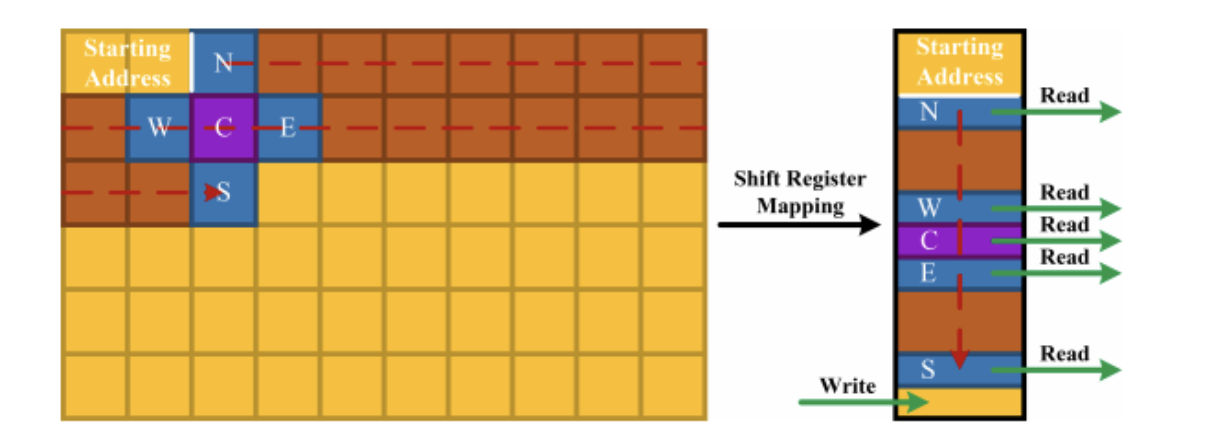
\includegraphics[width=0.6\textwidth]{Figures/slidingbuffer}
\decoRule
\caption[SlidingBuffer]{ Sliding Buffer Visualization. Source: \cite{2018combined}}
\label{fig:sliding buffer}
\end{figure}

\begin{figure}[h]
\centering
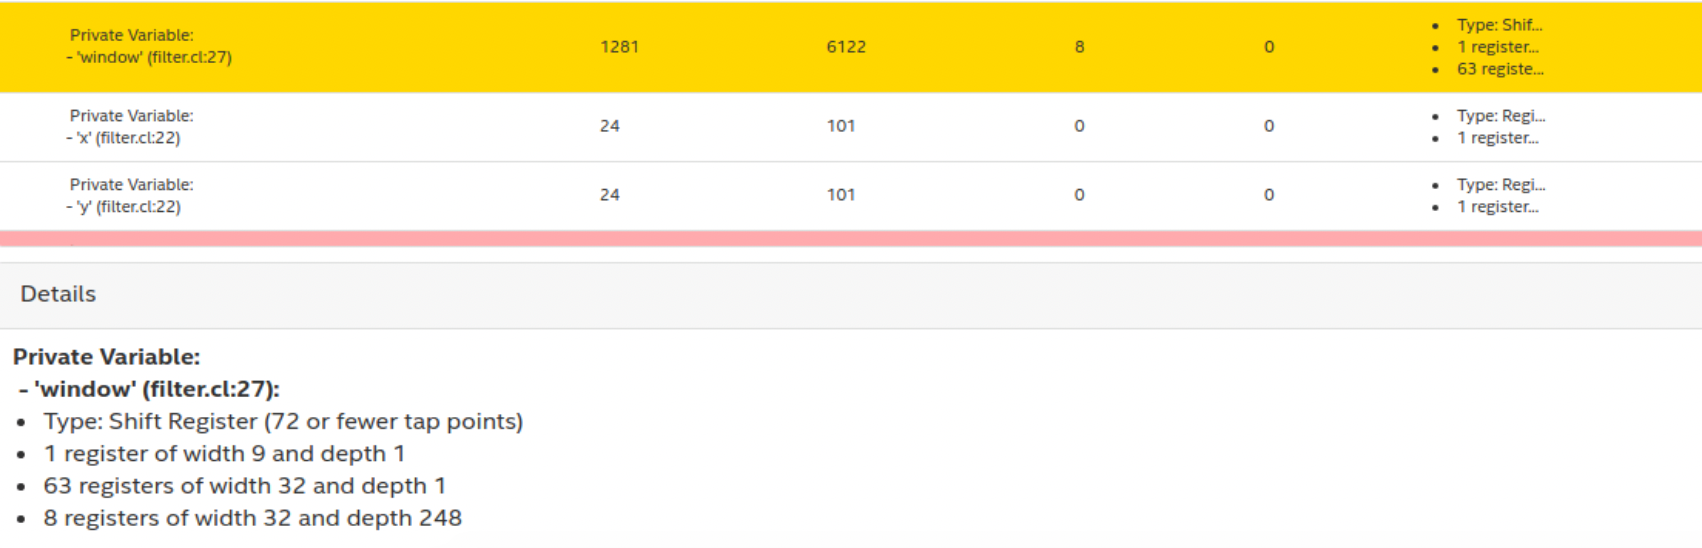
\includegraphics[width=1.0\textwidth]{Figures/shiftregister}
\decoRule
\caption[ShiftRegister]{ Sliding 'window' variable is inferred as a shift-register by the OpenCL compiler }
\label{fig:shiftregister}
\end{figure}

This implementation proves useful if data is provided in a streamlined fashion. The sliding buffer reads data sequentially and is more suitable for non-blocking dataflow computations.
\newline
\textbf{Limitations}
\newline
One of the limitations this implementation is that we quickly run out of buffer space as the dimensions of the problem grow larger. The sliding buffer size grows linearly with the above parameters: $ CH_{in}, Img_{w}, K_h, K_w $. For our application in a network as small as the Lenet, we do not worry about this problem. The solution to scaling the sliding buffer implementation is to utilize spatial blocking and tile the input into blocks and perform the computations in these tiles separately \cite{2018combined}.

\subsubsection{Row-stationary Implementation}

\begin{figure}[h]
\centering
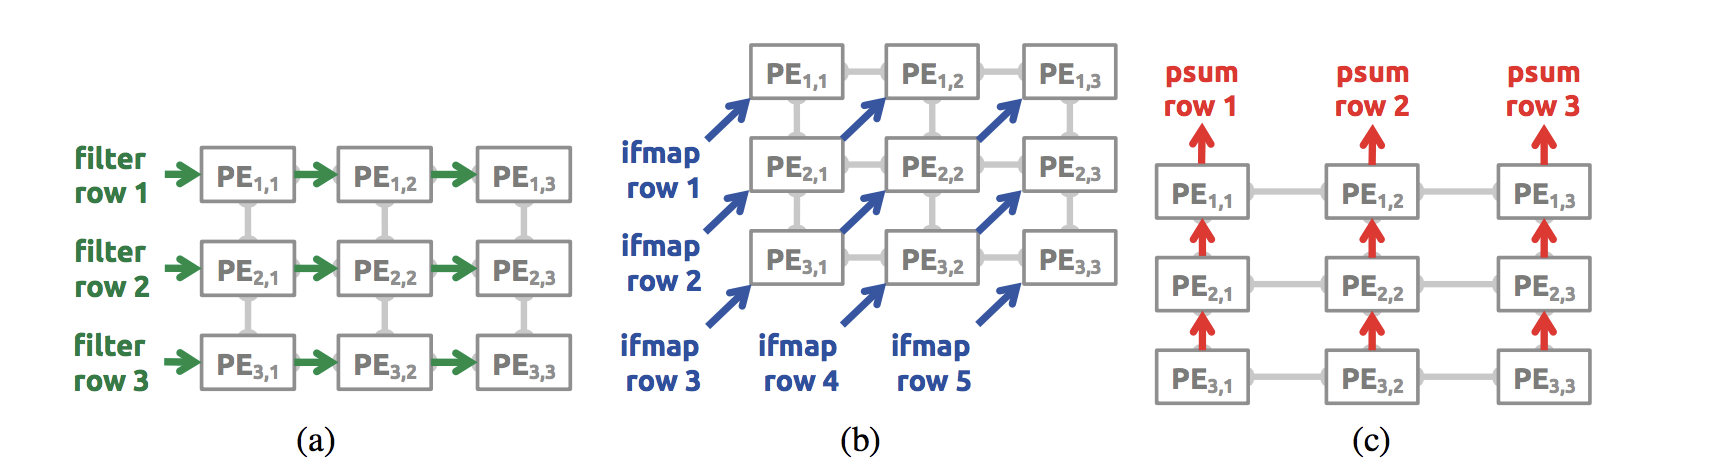
\includegraphics[width=1.0\textwidth]{Figures/eyeriss}
\decoRule
\caption[Eyeriss]{ Datar re-use across processing elements in Eyeriss. Source: \cite{eyeriss}}
\label{fig:eyeriss}
\end{figure}

\begin{figure}[h]
\centering
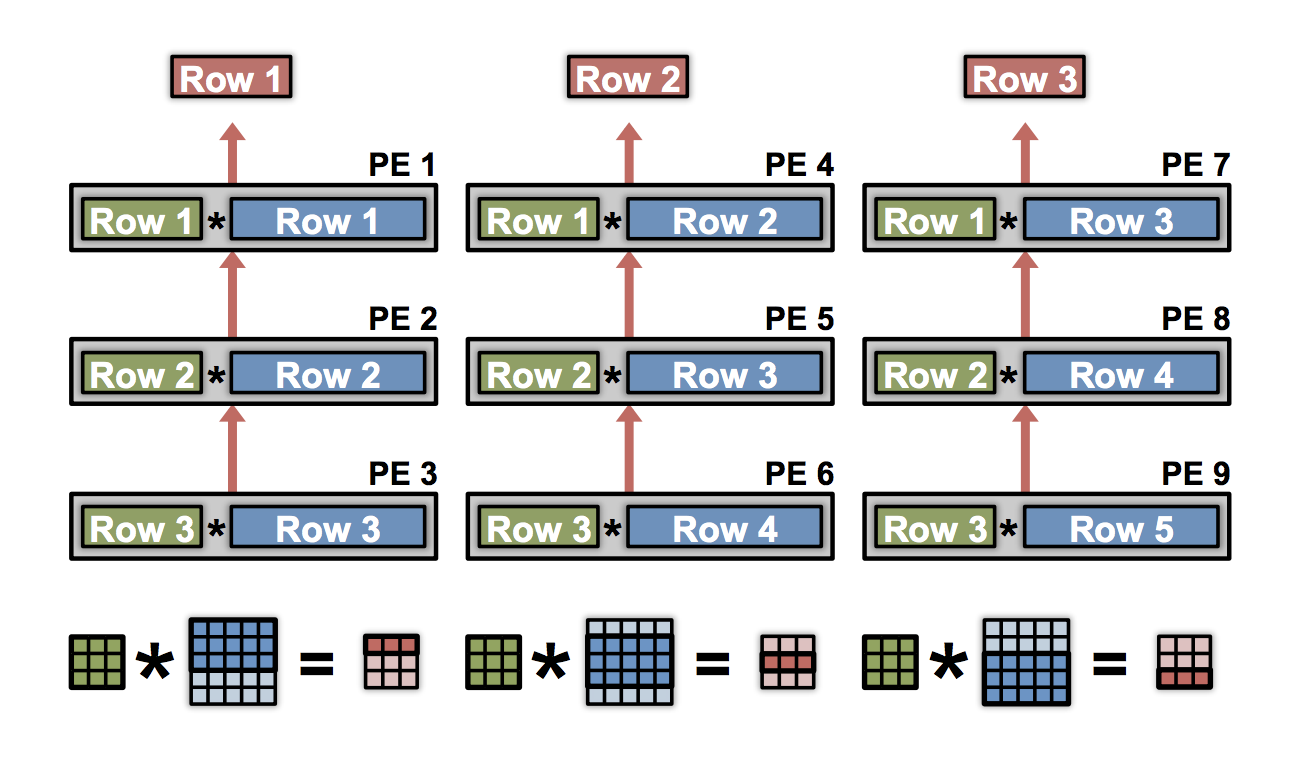
\includegraphics[width=0.6\textwidth]{Figures/eyeriss2}
\decoRule
\caption[Eyeriss2]{ 2D spatial convolution with a grid of processing elements (Eyeriss). Source: \cite{sze2017efficient}}
\label{fig:eyeriss2}
\end{figure}

This approach was suggested by Chen. et. al \cite{eyeriss} and it presents a way of reusing both filter weights and input feature maps. The technique requires a set of replicated processing unit. In the simple case of 3x3 filters we can instantiate 9 processing elements (PEs) each holding one of the 3x3 filter weights \ref{fig:eyeriss}. We implemented a simplified version of this architecture using the Intel SDK’s autorun kernels, which means the kernels do not need to be explicitly invoked and can communicate data to each other using channels ( FIFOs ). Input feature maps are then streamed diagonally (blue \ref{fig:eyeriss}) where they are required for the computation of different output feature map rows. The partial sums are accumulated upwards vertically ( shown in red \ref{fig:eyeriss} ) upwards. 

Advantages of using this is that the size of this grid can be adjusted to best fit the resources available on a specific board. This dataflow performs the theoretical minimum of memory reads required as input fmaps are read once and communicated diagonally to other PUs based on demand. Communication between PEs is done through Intel OpenCL channels which are Intel’s implmentation of FIFOs ( or pipes in OpenCL terms ) and computations are performed asynchronously. Two separate reader and writer kernels handle reading and writing data between global memory and the processing grid. The size of this grid is reconfigurable and the user can instantiate a larger version of this grid. It is independant of the image and filter sizes as we reuse techniques from Eyeriss \cite{eyeriss} such as folding and replication to map different computations onto the same fixed grid.


\subsubsection{Other Implementations}

The below methods were \textbf{not implemented} but it is worth discussing other approaches to performing a convolution. The shared idea is to transform the convolution operation into another form of computation with different properties thus allowing to perform different types of optimizations. 

\textbf{Matrix Multiplication:} One solution to the convolution problem involves transforming the input matrix and incorporating redundant data as in \cite{cudnn}. This transforms the convolution operation into a direct matrix multiplication. The downside of using this is the requirement of either a larger storage for storing the redundant inputs or a very complicated memory access pattern to be implemented \cite{ddl}.

\textbf{Fast-Fourier Transform (FFT):} Another solution is found by transitioning into the Fourier domain and applying a fourier transform on both the filter and the input image \cite{vasilache2014fast}. In the Fourier domain, a convolution becomes again a matrix multiplication. After multiplication of the frequency domain representations of the filter and the input, we use the inverse-fourier transform to obtain the output image. The fourier-transform decreases the complexity of the convolution operation from $ O(N_o^2N_f^2) $ to $ O(N_o^2log_2(N_o) $ where the input image size is $ N_oxN_o$ and the filter size is $ N_fxN_f $ .The tradeoff in this case is less operations on the expense of additional bandwidth and storage requirements. The quality of this transformation and benefits degrade for smaller filters and thus fourier is usally used in the case when large input features and filters are required \cite{sze2017efficient}. 

\textbf{Strassen's Algorithm}\cite{cong2014minimizing}: can reduce the number of multiplications from $O(N^3)$ to $O(N^{2.8})$\cite{sze2017efficient} . The reduced multiplications lower the space requirement as floating point operators require more space than additions but comes at the expense of numerical stability and storage space requirement to hold and propagate intermediate results \cite{sze2017efficient}.

\subsection{Maxpool Layer}


\section{OpenCL Kernel Template Generator}

\section{Integration with Deep500}